\documentclass[11pt
  , a4paper
  , article
  , oneside
  %  , twoside
  , showtrims
 % , draft
]{memoir}

\usepackage{essdocs}
\usepackage[numbers]{natbib}
\usepackage[autostyle]{csquotes}

\setsecnumdepth{subsection}


\begin{document}
%\frontmatter
% ESS Document Description
%
\essdoctype{Engineering Manual}

% ESS Document Number
%
\essdocnum{ESS-0064948}

% Date
%
\date{\today}

% ESS Document Revision Number
%
\essdocrev{1}

% ESS Document State
%
\essdocstate{Released}

% ESS Document Classification
%
\essdocclass{Internal}

% Document Title
%
\title{ICS Engineering Manual}
\subtitle{for MRF PCIe-EVR-300DC}
% Document Author(s), if more than one author,
% use \newline instead of \\ or \linebreak in order to seperate them
\author{Javier Cereijo Garcia \newline Jeong Han Lee}
\authorrole{Timing System Engineer \newline Senior Controls Engineer}

% Document Reviewer(s) if more than one reviewer,
% use \newline instead of \\ or \linebreak in order to seperate them
%\reviewer{-}
%\reviewerrole{-}

% Document Owner(s) if more than one owner,
% use \newline instead of \\ or \linebreak in order to seperate them
\owner{Javier Cereijo Garcia}
\ownerrole{Timing System Engineer}

% Document Approver(s) if more than one approver,
% use \newline instead of \\ or \linebreak in order to seperate them
%\approver{-}
%\approverrole{-}


\showtrimson

\esstitle
\newpage
\tableofcontents
\newpage

%\mainmatter


% Actual Document Start at below
\chapter{Overview}
At European Spallation Source (ESS), the Integrated Control System (ICS) uses the Micro-Research Finland (MRF) timing System{\footnote{\url{http://www.mrf.fi/}}} as its timing system of the ESS site. The consistent and up-to-date engineering manual is essential for the ESS timing system.\\


\section{Scope}
\begin{itemize}
\item This document identifies one of the MRF timing Event Receivers (EVRs) that needs to be configured for an ESS subsystem that needs synchronous frequencies, trigger signals and sequences of events \cite{MRFEVENTSYSTEMDC}.
\item This document provides the generic description of the MRF PCIe-EVR-300DC and its interface board (IFB-300). In addition, it affords the minimal, essential, and generic information for the system configuration.
\item The purpose of this document is to describe the engineering procedure and troubleshooting about how the MRF PCIe-EVR-300DC board will be integrated in cooperation with the new ESS EPICS Environment (E3).
\item This document attempts to maintain consistency with existing ESS timing system hardware as far as possible.
\end{itemize}
%\textbf{Note that this is a very early draft document and should be updated as development progresses.}


\section{Target audience}
This document is targeted to ICS engineers and technical stakeholders of the ESS timing system. It is assumed that the target audience has a technical background in the MRF timing system, the Experimental Physics and Industrial Control System (EPICS) development, and a Linux environment.\\


\chapter{System description}
MRF Technical Reference \citep[see][p45]{MRFEVENTSYSTEMDC} describes EVRs as:
\blockquote{\textit{Event Receivers decode timing events and signals from an optical event stream transmitted by an Event Generator. Events and signals are received at predefined rate the event clock that is usually divided down from an accelerators main RF reference. The event receivers lock to the phase event clock of the Event Generator and are thus phase locked to the RF reference. Event Receivers convert event codes transmitted by an Event Generator to hardware outputs. They can also generate software interrupts and store the event codes with globally distributed timestamps into FIFO memory to be read by a CPU.}}

ICS uses and will use the following different types of EVRs:
\begin{itemize}
\item mTCA-EVR-300(U)
\item PCIe-EVR-300DC
\end{itemize}

The scope of this document is to cover PCIe-EVR-300DC board.\\


\section{PCIe-EVR-300DC}
Figure~\ref{fig:pcie-evr300dc} shows the rough physical dimensions $104\times 79~\mathrm{mm}{}^2$ of the PCIe-EVR-300DC card. Its power dissipation is almost 10W, so it is necessary to check the maximum power that the PCIe slot where the EVR will be installed is capable of providing.. It is also advisable to have some forced cooling method to keep the temperature of the card reasonable \citetext{priv. comm.}.\\

\begin{figure}[!htb]
  \centering
  \includegraphics[width=0.99\textwidth]{./pictures/pcie_evr_300dc.eps}
  \caption{
    MRF PCIe-EVR-300DC.
  }
  \label{fig:pcie-evr300dc}
\end{figure}


The PCIe-EVR-300DC  has a small form-factor pluggable (SFP) transceiver as an input from an Event Master (EVM) and a micro-SCSI type connector for an interface board IFB-300. The IFB-300 has 8 Universal Input/Output (I/O) slots, each of them accommodating 2 outputs/inputs, shown in Figure~\ref{fig:ifb-300}. With different types of MRF Universal I/O modules, each slot can be used as an unique trigger or event signal source.\\

\begin{figure}[!htb]
  \centering
  \includegraphics{./pictures/ifb-300.eps}
  \caption{
    MRF Interface Board IFB 300 Front Panel \cite{MRFEVENTSYSTEMDC}.
  }
  \label{fig:ifb-300}
\end{figure}



%\clearpage
\chapter{System environment}
Before describing the engineering procedure for the E3 integration of the MRF PCIe-EVR-300DC board, it is mandatory to have a proper system environment that consists of specific hardware and software. Here we will show the hardware and software lists and their set up in the ICS lab at ESS. The information shown in this chapter is used in the ICS lab at ESS.\\

\section{Hardware}
Table~\ref{table:hwlist} shows the hardware list. It is possible to use a different form factor for the EVM than what is shown; for more information check the specific engineering manual. It is assumed that a working EVM system is ready. The Advantech Industrial PC can be replaced with any other type of Industrial PC (IPC), workstation or server with a compatible PCIe slot. Note that this PCIe slot for the MRF PCIe-EVR-300DC should support more than 10W.
\begin{table}[!hb]
  \centering
  \begin{tabular}{l|l}
    \toprule
    Hardware                          & Info                      \\\midrule
    MRF PCIe-EVR-300DC                &                           \\\midrule
    Advantech Industrial PC           &                           \\\midrule
    MRF IFB-300                       & Inc. cable                \\\midrule
    Universal I/O                     &                           \\\midrule
    MRF mTCA-EVM-300                  & Inc. $\mu$TCA crate, etc  \\\midrule
    Ethernet, LEMO and optical cables & LC, Optical 850 nm        \\\midrule
    Oscilloscope                      &                           \\\bottomrule
  \end{tabular}
  \caption[]{Hardware List and Its Environment.}
  \label{table:hwlist}
\end{table}

Figure~\ref{fig:ipc} shows the IPC with two PCIe-EVR-300DC installed. The IFB-300 is not shown in the figure.\\

\begin{figure}[!b]
  \centering
  \includegraphics[width=0.8\textwidth]{./pictures/ipc.jpg}
  \caption{IPC with two PCIe-EVR-300DC installed.}
  \label{fig:ipc}
\end{figure}


%\clearpage
\section{Software}
Table~\ref{table:swlist} shows the software list and its environment.

\begin{table}[!htb]
  \centering
  \begin{tabular}{l|l}
    \toprule
    Item               & Version Info.                                                       \\\midrule
    CentOS Linux       & \texttt{7.7.1908}                                                  \\\midrule
    Kernel             & \texttt{3.10.0-1062.9.1.el7.x86\_64}                               \\\midrule
    mrf kernel module  & Version: \texttt{1} / srcversion \texttt{E3290AD048B5B57D2EAA55E}  \\\midrule
    EPICS base         & \texttt{7.0.3.1}                                                   \\\midrule
    e3-req             & \texttt{3.1.2}                                                     \\\midrule
    mrfioc2            & E3 module ver. \texttt{2.2.0-rc8}                                  \\\midrule
    devLib2            & E3 module ver. \texttt{2.9.0}                                      \\\bottomrule
  \end{tabular}
  \caption[]{Software and its version information.}
  \label{table:swlist}
\end{table}

\section{EVR firmware}
Table~\ref{table:fwinfo} shows the EVR field-programmable gate array (FPGA) Firmware Version Register.

\begin{table}[!htb]
  \centering
  \begin{tabular}{p{0.3\linewidth}|c|l}
    \toprule
    EVR FPGA Firmware Version Register              & \multicolumn{2}{c}{\texttt{0x17080207}}             \\\midrule
    Board Type        & EVR                         &  \texttt{0x}\underline{\textbf{1}}\texttt{7080207}  \\\midrule
    Form Factor       & PCIe                        &  \texttt{0x1}\underline{\textbf{7}}\texttt{080207}  \\\midrule
    EVR Subrelease ID & 8                           &  \texttt{0x17}\underline{\textbf{08}}\texttt{0207}  \\\midrule
    EVR Firmware ID   & Delay Compensation Firmware &  \texttt{0x1708}\underline{\textbf{02}}\texttt{07}  \\\midrule
    EVR Revision ID   & 7                           &  \texttt{0x170802}\underline{\textbf{07}}           \\\bottomrule
  \end{tabular}
  \caption[]{EVR FPGA Firmware Version Register in Reference \citep[see][p66]{MRFEVENTSYSTEMDC}.}
  \label{table:fwinfo}
\end{table}


%\clearpage
\chapter{Engineering procedure}
This chapter provides the minimal information to configure the EVR board properly.\\

\section{System installation}
Figure~\ref{fig:ipc} shows a glimpse of what the system might look like in the lab. \textbf{Note that the cable between the PCIe-EVR-300DC and the IFB-300 should be connected or disconnected only when the system is powered down}. Please see more detailed information in \citep[][p54]{MRFEVENTSYSTEMDC}.\\

It is assumed that the IPC is running CentOS 7 with E3. For more information on E3, please check {\footnote{\url{https://github.com/icshwi/e3training}}.\\


\section{PCIe-EVR-300DC Board Identification}

\subsection{Fixing PCI IDs}
The PCI ID list does not include the MRF products. It can be updated as follows:
\begin{itemize}
\item Clone the customized PCI.IDS database with the MRF products:
\begin{lstlisting}[style=termstyle]
iocuser@icslab-ipc01: ics_gitsrc$ git clone https://github.com/jeonghanlee/pciids
\end{lstlisting}
\item Replace the pci.ids file:
\begin{lstlisting}[style=termstyle]
iocuser@icslab-ipc01: pciids (master)$ bash replace-pciids.bash
centos was determined.
[sudo] password for iocuser:
\end{lstlisting}
\item Check MRF products by the vendor's id (1a3e):
\begin{lstlisting}[style=termstyle]
iocuser@icslab-ipc01: pciids (master)$ lspci -nmmn | grep -E "\<(1a3e)"
02:00.0 "Signal processing controller [1180]" "Xilinx Corporation [10ee]" "XILINX PCI DEVICE [7011]" "Micro-Research Finland Oy [1a3e]" "PCIE Event Receiver 300(DC) [172c]"
\end{lstlisting}
\end{itemize}

\subsection{Kernel module}
The PCIE-EVR-300DC needs a kernel module to work. It can be installed by simply running some commands. Do the following:
\begin{itemize}
\item Go to your e3-mrfioc2 sources directory:
\begin{lstlisting}[style=termstyle]
iocuser@icslab-ipc01: ~$ cd e3/e3-mrfioc2
\end{lstlisting}
\item Install the kernel module:
\begin{lstlisting}[style=termstyle]
iocuser@icslab-ipc01: e3-mrfioc2 (master)$ make dkms_add
/epics/base-7.0.3.1/bin/linux-x86_64/msi -M name="mrfioc2" -M  version="2.2.0-rc8" -M kmod_name="mrf" /home/iocuser/e3/e3-mrfioc2/dkms/dkms_with_msi.conf.in > /home/iocuser/e3/e3-mrfioc2/dkms/dkms_with_msi.conf
/usr/bin/sudo -E install -d /usr/src/mrfioc2-2.2.0-rc8
[sudo] password for iocuser:
/usr/bin/sudo -E cp -r /home/iocuser/e3/e3-mrfioc2/mrfioc2/mrmShared/linux/* /usr/src/mrfioc2-2.2.0-rc8/
/usr/bin/sudo -E /usr/sbin/dkms add -m mrfioc2 -v 2.2.0-rc8

Creating symlink /var/lib/dkms/mrfioc2/2.2.0-rc8/source ->
                 /usr/src/mrfioc2-2.2.0-rc8

DKMS: add completed.
iocuser@icslab-ipc01: e3-mrfioc2 (master)$ make dkms_build
/usr/bin/sudo -E /usr/sbin/dkms build -m mrfioc2 -v 2.2.0-rc8

Kernel preparation unnecessary for this kernel.  Skipping...

Building module:
cleaning build area...
make -j4 KERNELRELEASE=3.10.0-1062.9.1.el7.x86_64 -C /lib/modules/3.10.0-1062.9.1.el7.x86_64/build M=/var/lib/dkms/mrfioc2/2.2.0-rc8/build modules...
cleaning build area...

DKMS: build completed.
iocuser@icslab-ipc01: e3-mrfioc2 (master)$ make dkms_install
/usr/bin/sudo -E /usr/sbin/dkms install -m mrfioc2 -v 2.2.0-rc8

mrf.ko.xz:
Running module version sanity check.
 - Original module
   - No original module exists within this kernel
 - Installation
   - Installing to /lib/modules/3.10.0-1062.9.1.el7.x86_64/extra/
Adding any weak-modules

depmod...

DKMS: install completed.
iocuser@icslab-ipc01: e3-mrfioc2 (master)$ make setup
KERNEL=="uio*", ATTR{name}=="mrf-pci", MODE="0666"
mrf
rmmod mrf
rmmod parport
rmmod uio
insmod /lib/modules/3.10.0-1062.9.1.el7.x86_64/kernel/drivers/parport/parport.ko.xz
insmod /lib/modules/3.10.0-1062.9.1.el7.x86_64/kernel/drivers/uio/uio.ko.xz
insmod /lib/modules/3.10.0-1062.9.1.el7.x86_64/extra/mrf.ko.xz


It is OK to see "E3/RULES_DKMS:37: recipe for target 'setup' failed"
---------------------------------------------------------------------
crw-rw-rw- 1 root root 245, 0 Feb 04 15:37 /dev/uio0
crw-rw-rw- 1 root root 245, 1 Feb 04 15:37 /dev/uio1
---------------------------------------------------------------------
\end{lstlisting}
\item Check kernel module information:
\begin{lstlisting}[style=termstyle]
iocuser@icslab-ipc01: e3-mrfioc2 (master)$ lsmod |grep mrf
mrf                    18137  0
parport                46395  1 mrf
uio                    19338  1 mrf
iocuser@icslab-ipc01: e3-mrfioc2 (master)$ modinfo mrf
filename:       /lib/modules/3.10.0-1062.9.1.el7.x86_64/extra/mrf.ko.xz
author:         Michael Davidsaver <mdavidsaver@gmail.com>
version:        1
license:        GPL v2
retpoline:      Y
rhelversion:    7.7
srcversion:     E3290AD048B5B57D2EAA55E
alias:          pci:v000010EEd00007011sv00001A3Esd0000232Cbc*sc*i*
alias:          pci:v000010EEd00007011sv00001A3Esd0000132Cbc*sc*i*
alias:          pci:v00001A3Ed0000152Csv00001A3Esd0000152Cbc*sc*i*
alias:          pci:v00001A3Ed0000252Csv00001A3Esd0000252Cbc*sc*i*
alias:          pci:v000010EEd00007011sv00001A3Esd0000172Cbc*sc*i*
alias:          pci:v00001204d0000EC30sv00001A3Esd0000172Cbc*sc*i*
alias:          pci:v000010B5d00009056sv00001A3Esd0000192Cbc*sc*i*
alias:          pci:v000010B5d00009030sv00001A3Esd000011E6bc*sc*i*
alias:          pci:v000010B5d00009030sv00001A3Esd000020E6bc*sc*i*
alias:          pci:v000010B5d00009030sv00001A3Esd000020DCbc*sc*i*
alias:          pci:v000010B5d00009030sv00001A3Esd000010E6bc*sc*i*
depends:        parport,uio
vermagic:       3.10.0-1062.9.1.el7.x86_64 SMP mod_unload modversions
parm:           cable:Name of JTAG parallel port cable to emulate (charp)
parm:           interfaceversion:User space interface version (int)
parm:           use_msi:Use MSI if present (default 1, yes) (uint)

\end{lstlisting}
%Check that the source version is the same as shown; it should be if these steps are followed as shown. Otherwise please inform ICS.
\end{itemize}


\subsection{PCI addressing}
Each PCI device is identified by a domain, a bus, a device, and a function number in Linux. Therefore, in order to initialize the MRF PCIe-EVR-300DC board in E3, one needs the following information: a bus number, a device number, and a function number. These numbers are the parameters of a \texttt{mrmEvrSetupPCI} function.\\

One can use \texttt{lspci} to find them as follows:
\begin{lstlisting}[style=termstyle]
iocuser@icslab-ipc01: e3-mrfioc2 (master)$ lspci
[...]
02:00.0 Signal processing controller: Xilinx Corporation XILINX PCI DEVICE
[...]
iocuser@icslab-ipc01: e3-mrfioc2 (master)$ lspci -s 02:00.0 -vv
02:00.0 Signal processing controller: Xilinx Corporation XILINX PCI DEVICE
	Subsystem: Micro-Research Finland Oy PCIE Event Receiver 300(DC)
	Control: I/O+ Mem+ BusMaster+ SpecCycle- MemWINV- VGASnoop- ParErr- Stepping- SERR- FastB2B- DisINTx+
	Status: Cap+ 66MHz- UDF- FastB2B- ParErr- DEVSEL=fast >TAbort- <TAbort- <MAbort- >SERR- <PERR- INTx-
	Latency: 0
	Interrupt: pin A routed to IRQ 337
	Region 0: Memory at df300000 (32-bit, non-prefetchable) [size=256K]
	Capabilities: <access denied>
	Kernel driver in use: mrf-pci
	Kernel modules: mrf

\end{lstlisting}

And one should identify four number as follows:
\begin{lstlisting}[style=termstyle]
iocuser@icslab-ipc01: e3-mrfioc2 (master)$ lspci -s 02:00.0 -t
-+-[0000:02]---00.0
 \-[0000:00]-
\end{lstlisting}
, where \texttt{-+-[0000:02]---00.0} can be translated to \texttt{-+-}[domain:bus]\texttt{---}device.function. Thus for the case above the numbers are shown in Table~\ref{table:pciidnumber}.\begin{table}[!htb]
  \centering
  \begin{tabular}{l|l}
    \toprule
    bus      & 0x2 \\\midrule
    device   & 0x0 \\\midrule
    function & 0x0 \\\bottomrule
  \end{tabular}
  \caption[]{MRF PCIe-EVR-300DC Identification Numbers}
  \label{table:pciidnumber}
\end{table}


%\clearpage
\section{EPICS IOC set up under E3}
In order to start the EPICS Input/Output Controller (IOC) for the MRF PCIE-EVR-300DC under E3, one should consider two things: 1) the EPICS database file, and 2) the EPICS start-up script. Let us set as the working directory,
\begin{lstlisting}[style=termstyle, label={list:pwd}, caption={Working directory in the ICS lab.} ]
/home/iocuser/e3/e3-mrfioc2/cmds
\end{lstlisting}

\subsection{EPICS database file}
The database files in E3 are located under the following directory:
\begin{lstlisting}[style=termstyle]
/epics/base-7.0.3.1/require/3.1.2/siteMods/mrfioc2/2.2.0-rc8/db/evr-pcie-300dc-ess.db
\end{lstlisting}

\subsection{Start-up script}
Listing~\ref{list:empcieevr300dc.cmd} shows the IOC start-up script configured for the MRF PCIE-EVR-300DC present in our system with the Identification Numbers obtained in previous steps.
\begin{lstlisting}[
    style=termstyle,
    numbers=left,
    label={list:empcieevr300dc.cmd},
    caption={Start-up script \texttt{empcieevr300dc.cmd}. Line \ref{pciid0} should be matched to Table~\ref{table:pciidnumber} as \texttt{mrmEvrSetupPCI(\$(DEV1), "bus:device.function")}.}
  ]
require mrfioc2,2.2.0-rc8

epicsEnvSet("IOC", "EMPCIEEVR300DC")
epicsEnvSet("DEV1", "EVR0")

epicsEnvSet("MainEvtCODE" "14")
epicsEnvSet("HeartBeatEvtCODE"   "122")
epicsEnvSet("ESSEvtClockRate"  "88.0525")

mrmEvrSetupPCI("$(DEV1)",  "0a:00.0")(*@\label{pciid0}@*)
dbLoadRecords("evr-pcie-300dc-ess.db","EVR=$(DEV1), SYS=$(IOC), D=$(DEV1), FEVT=$(ESSEvtClockRate), EVNT1HZ=$(MainEvtCODE)")

var evrMrmTimeNSOverflowThreshold 100000


iocInit()

\end{lstlisting}


\subsection{EPICS IOC}
All the EPICS parameters should be run from an E3 session. To start E3, type:
\begin{lstlisting}[style=termstyle]
iocuser@icslab-ipc01: cmds (master)$ source /epics/base-7.0.3.1/require/3.1.2/bin/setE3Env.bash

Set the ESS EPICS Environment as follows:
THIS Source NAME    : setE3Env.bash
THIS Source PATH    : /epics/base-7.0.3.1/require/3.1.2/bin
EPICS_BASE          : /epics/base-7.0.3.1
EPICS_HOST_ARCH     : linux-x86_64
E3_REQUIRE_LOCATION : /epics/base-7.0.3.1/require/3.1.2
PATH                : /epics/base-7.0.3.1/require/3.1.2/bin:/epics/base-7.0.3.1/bin/linux-x86_64:/usr/local/bin:/usr/bin:/usr/local/sbin:/usr/sbin:/home/iocuser/.local/bin:/home/iocuser/bin
LD_LIBRARY_PATH     : /epics/base-7.0.3.1/lib/linux-x86_64:/epics/base-7.0.3.1/require/3.1.2/lib/linux-x86_64:/epics/base-7.0.3.1/require/3.1.2/siteLibs/linux-x86_64

Enjoy E3!
\end{lstlisting}
All the IOCs and related EPICS commands (caget, caput, camonitor, etc.) should be run from an E3 session.\\

Under E3, the EPICS IOC can be started with the command \texttt{iocsh.bash empcieevr300dc.cmd}. The output should look like as follows:
\begin{lstlisting}[style=termstyle]
iocuser@icslab-ipc01: cmds (master)$ iocsh.bash empcieevr300dc.cmd
registerChannelProviderLocal firstTime true
#
# ------>-----> snip ----->------>
#
# Please Use Version and other environment variables
# in order to report or debug this shell
#
# The IOC is started at "2020-W06-Feb04-1644-58-CET"
#
# Version information:
# European Spallation Source ERIC : iocsh.bash (0.5.1-81d1214.PID-24674)
#
# HOSTDISPLAY=""
# WINDOWID=""
# PWD="/home/iocuser/e3/e3-mrfioc2/cmds"
# USER="iocuser"
# LOGNAME="iocuser"
# EPICS_HOST_ARCH="linux-x86_64"
# EPICS_BASE="/epics/base-7.0.3.1"
# E3_REQUIRE_NAME="require"
# E3_REQUIRE_VERSION="3.1.2"
# E3_REQUIRE_LOCATION="/epics/base-7.0.3.1/require/3.1.2"
# E3_REQUIRE_BIN="/epics/base-7.0.3.1/require/3.1.2/bin"
# E3_REQUIRE_DB="/epics/base-7.0.3.1/require/3.1.2/db"
# E3_REQUIRE_DBD="/epics/base-7.0.3.1/require/3.1.2/dbd"
# E3_REQUIRE_INC="/epics/base-7.0.3.1/require/3.1.2/include"
# E3_REQUIRE_LIB="/epics/base-7.0.3.1/require/3.1.2/lib"
# E3_SITEAPPS_PATH="/epics/base-7.0.3.1/require/3.1.2/siteApps"
# E3_SITELIBS_PATH="/epics/base-7.0.3.1/require/3.1.2/siteLibs"
# E3_SITEMODS_PATH="/epics/base-7.0.3.1/require/3.1.2/siteMods"
# EPICS_DRIVER_PATH="/epics/base-7.0.3.1/require/3.1.2/siteMods:/epics/base-7.0.3.1/require/3.1.2/siteApps"
# EPICS_CA_AUTO_ADDR_LIST=""
# EPICS_CA_ADDR_LIST=""
# PATH="/epics/base-7.0.3.1/require/3.1.2/bin:/epics/base-7.0.3.1/bin/linux-x86_64:/usr/local/bin:/usr/bin:/usr/local/sbin:/usr/sbin:/home/iocuser/.local/bin:/home/iocuser/bin"
# LD_LIBRARY_PATH="/epics/base-7.0.3.1/lib/linux-x86_64:/epics/base-7.0.3.1/require/3.1.2/lib/linux-x86_64:/epics/base-7.0.3.1/require/3.1.2/siteLibs/linux-x86_64"
#
# ------>-----> snip ----->------>
#
# Set REQUIRE_IOC for its internal PVs
epicsEnvSet REQUIRE_IOC "REQMOD:81d1214-cslab-c-24674"
#
# Enable an exit subroutine.
dbLoadRecords "/epics/base-7.0.3.1/db/softIocExit.db" "IOC=REQMOD:81d1214-cslab-c-24674"
#
# Set E3_IOCSH_TOP for the absolute path where iocsh.bash is executed.
epicsEnvSet E3_IOCSH_TOP "/home/iocuser/e3/e3-mrfioc2/cmds"
#
# Load require module, which has the version 3.1.2
#
dlload /epics/base-7.0.3.1/require/3.1.2/lib/linux-x86_64/librequire.so
dbLoadDatabase /epics/base-7.0.3.1/require/3.1.2/dbd/require.dbd
require_registerRecordDeviceDriver
Loading module info records for require
#
# Set E3_CMD_TOP for the absolute path where empcieevr300dc.cmd exists
epicsEnvSet E3_CMD_TOP "/home/iocuser/e3/e3-mrfioc2/cmds"
#
iocshLoad 'empcieevr300dc.cmd',''
require mrfioc2,2.2.0-rc8
Module mrfioc2 version 2.2.0-rc8 found in /epics/base-7.0.3.1/require/3.1.2/siteMods/mrfioc2/2.2.0-rc8/
Module mrfioc2 depends on devlib2 2.9.0
Module devlib2 version 2.9.0 found in /epics/base-7.0.3.1/require/3.1.2/siteMods/devlib2/2.9.0/
Loading library /epics/base-7.0.3.1/require/3.1.2/siteMods/devlib2/2.9.0/lib/linux-x86_64/libdevlib2.so
Loaded devlib2 version 2.9.0
Loading dbd file /epics/base-7.0.3.1/require/3.1.2/siteMods/devlib2/2.9.0/dbd/devlib2.dbd
Calling function devlib2_registerRecordDeviceDriver
Loading module info records for devlib2
Loading library /epics/base-7.0.3.1/require/3.1.2/siteMods/mrfioc2/2.2.0-rc8/lib/linux-x86_64/libmrfioc2.so
Loaded mrfioc2 version 2.2.0-rc8
Loading dbd file /epics/base-7.0.3.1/require/3.1.2/siteMods/mrfioc2/2.2.0-rc8/dbd/mrfioc2.dbd
Calling function mrfioc2_registerRecordDeviceDriver
Loading module info records for mrfioc2
epicsEnvSet("IOC", "EMPCIEEVR300DC")
epicsEnvSet("DEV1", "EVR0")
#epicsEnvSet("MainEvtCODE" "14")
#epicsEnvSet("HeartBeatEvtCODE"   "122")
epicsEnvSet("ESSEvtClockRate"  "88.0525")
mrmEvrSetupPCI("EVR0",  "02:00.0")
Notice: devPCIFindSpec() expect B:D.F in hex
Device EVR0  2:0.0 slot=(null)
Using IRQ 337
FWVersion 0x17080207
Found version 519
Found SFP EEPROM
Sequencer capability detected
PCIe: Out FP:0 FPUNIV:16 RB:0 IFP:16 GPIO:0
Enabling interrupts
dbLoadRecords("evr-pcie-300dc-ess.db","EVR=EVR0, SYS=EMPCIEEVR300DC, D=EVR0, FEVT=88.0525, EVNT1HZ=14")
EVR FIFO task start
var evrMrmTimeNSOverflowThreshold 100000
iocInit()
Starting iocInit
############################################################################
## EPICS R7.0.3.1-E3-7.0.3.1-patch
## EPICS Base built Jan 28 2020
############################################################################
Set EVR clock 88052500.000000
iocRun: All initialization complete
# Set the IOC Prompt String One
epicsEnvSet IOCSH_PS1 "81d1214-cslab-c-24674 > "
#
81d1214-cslab-c-24674 >
\end{lstlisting}

In addition, the PCI information is available within the running IOC via \texttt{devPCIShow} as follows:
\begin{lstlisting}
81d1214-cslab-c-24674 > devPCIShow
\end{lstlisting}
Look for the line with your configuration information, in our case is:
\begin{lstlisting}
PCI 0000:02:00.0 IRQ 337
  vendor:device 10ee:7011 rev 00
\end{lstlisting}
Where the vendor id \texttt{10ee} is \texttt{Xilinx Corporation}.\\

The PCI information can be shown with (the second parameter is the verbosity level):
\begin{lstlisting}
81d1214-cslab-c-24674 > devPCIShow 9 0x10ee
...
PCI 0000:02:00.0 IRQ 337
  vendor:device 10ee:7011 rev 00
  subved:subdev 1a3e:172c
  class 118000 generic signal processing controller
  driver mrf-pci
  BAR 0 32-bit MMIO    256 kB
...
\end{lstlisting}

\subsection{Checking automatic configuration after reboot}
Reboot and check that the module is loaded and the IOC correctly starts:
\begin{lstlisting}[style=termstyle]
iocuser@icslab-ipc01: ~$ lsmod |grep mrf
mrf                    18137  0
uio                    19338  1 mrf
parport                46395  1 mrf
\end{lstlisting}



%\newpage
\chapter{System in-situ verification and configuration procedure}
This chapter provides the minimal system verification procedure. If it is desired to perform a more detailed testing please see Reference~\citep[see][p14]{EVR-USER-GUIDE}. It also explains how to configure the EVR in deeper detail.

\begin{table}[!htb]
  \centering
  \begin{tabular}{c|p{0.4\linewidth}|p{0.42\linewidth}}
    \toprule
    Step & Goal                                       & Info.                                                  \\\midrule
    1    & Check the EVR \& EVM connection            & Link status, link clock, and heartbeat timeout counter \\\midrule
    2    & Monitor receiving and acknowledging events & Event counter and receiving event frequency            \\\midrule
    3    & Generate trigger signals from EVR          & Various trigger signals with an oscilloscope           \\\midrule
    4    & Configure hardware timestamps              & Timestamps from the EVM                                \\\midrule
    5    & Use the EVR in standalone mode             & Use the EVR without an EVM                             \\\midrule
    6    & Generate events from the inputs            & Use the inputs                                         \\\bottomrule
  \end{tabular}
  \caption[]{System in-situ verification procedure}
  \label{table:checklist}
\end{table}


\section{Step 1: Check the EVR and EVM connection}
This assumes that the EVR is connected to a properly configured EVM. Short comments on each command or a series of commands are shown before the corresponding command.
\begin{lstlisting}[style=termstyle]
#
# We can check the EVM and EVR link status and the link clock setting,
# and can also see the link counter
#
iocuser@icslab-ipc01: ~$ caget EMPCIEEVR300DC-EVR0:Link-Sts
EMPCIEEVR300DC-EVR0:Link-Sts     OK
iocuser@icslab-ipc01: ~$ caget EMPCIEEVR300DC-EVR0:Link-Clk-I
EMPCIEEVR300DC-EVR0:Link-Clk-I   88.0519
#
# Change the clock setting on the EVR, and check the link status turn to Fail
#
iocuser@icslab-ipc01: ~$ caput EMPCIEEVR300DC-EVR0:Link-Clk-SP 100
Old : EMPCIEEVR300DC-EVR0:Link-Clk-SP  88.0525
New : EMPCIEEVR300DC-EVR0:Link-Clk-SP  100
iocuser@icslab-ipc01: ~$ caget EMPCIEEVR300DC-EVR0:Link-Sts
EMPCIEEVR300DC-EVR0:Link-Sts     Fail
iocuser@icslab-ipc01: ~$ caget EMPCIEEVR300DC-EVR0:Link-Clk-I
EMPCIEEVR300DC-EVR0:Link-Clk-I   100
#
# Revert it back to the proper clock setting, and the link status will be OK
#
iocuser@icslab-ipc01: ~$ caput EMPCIEEVR300DC-EVR0:Link-Clk-SP 88.0525
Old : EMPCIEEVR300DC-EVR0:Link-Clk-SP  100
New : EMPCIEEVR300DC-EVR0:Link-Clk-SP  88.0525
iocuser@icslab-ipc01: ~$ caget EMPCIEEVR300DC-EVR0:Link-Sts
EMPCIEEVR300DC-EVR0:Link-Sts     OK
iocuser@icslab-ipc01: ~$ caget EMPCIEEVR300DC-EVR0:Link-Clk-I
EMPCIEEVR300DC-EVR0:Link-Clk-I   88.0519
#
# The link heartbeat counter is 35, depending on the time spent on Fail status
#
iocuser@icslab-ipc01: ~$ camonitor EMPCIEEVR300DC-EVR0:Cnt-LinkTimo-I
EMPCIEEVR300DC-EVR0:Cnt-LinkTimo-I 2020-02-05 14:59:19.909288 35
#
# Open another terminal to change the link clock
#
iocuser@icslab-ipc01: ~$ caput EMPCIEEVR300DC-EVR0:Link-Clk-SP 100
Old : EMPCIEEVR300DC-EVR0:Link-Clk-SP  88.0525
New : EMPCIEEVR300DC-EVR0:Link-Clk-SP  100
#
# In the original terminal the heartbeat counter should be increasing as follows:
#
EMPCIEEVR300DC-EVR0:Cnt-LinkTimo-I 2020-02-05 15:07:40.035069 36
EMPCIEEVR300DC-EVR0:Cnt-LinkTimo-I 2020-02-05 15:07:41.316697 37
EMPCIEEVR300DC-EVR0:Cnt-LinkTimo-I 2020-02-05 15:07:42.597370 38
EMPCIEEVR300DC-EVR0:Cnt-LinkTimo-I 2020-02-05 15:07:43.877849 39
EMPCIEEVR300DC-EVR0:Cnt-LinkTimo-I 2020-02-05 15:07:45.158539 40
#
# The counter will be stopped after the proper value is set again
#
# In the second terminal:
#
iocuser@icslab-ipc01: ~$ caput EMPCIEEVR300DC-EVR0:Link-Clk-SP 88.0525
Old : EMPCIEEVR300DC-EVR0:Link-Clk-SP  100
New : EMPCIEEVR300DC-EVR0:Link-Clk-SP  88.0525
#
# Check that the EVM is sending a timestamp
#
iocuser@icslab-ipc01: ~$ caget EMPCIEEVR300DC-EVR0:Time-Valid-Sts
EMPCIEEVR300DC-EVR0:Time-Valid-Sts Valid
\end{lstlisting}


\section{Step 2: Monitor receiving and acknowledging events}
This assumes that the EVM is sending event 14 at 14 Hz. Short comments on each command or a series of commands are shown before the corresponding command.
\begin{lstlisting}[style=termstylenumber]
#
# Set the EVR to log event 14 with event counter E
#
iocuser@icslab-ipc01: ~$ caput EMPCIEEVR300DC-EVR0:EvtE-SP.OUT "@OBJ=EVR0,Code=14"
Old : EMPCIEEVR300DC-EVR0:EvtE-SP.OUT        @OBJ=EVR0,Code=255
New : EMPCIEEVR300DC-EVR0:EvtE-SP.OUT        @OBJ=EVR0,Code=14
iocuser@icslab-ipc01: ~$ caput EMPCIEEVR300DC-EVR0:EvtE-SP 14
Old : EMPCIEEVR300DC-EVR0:EvtE-SP            255
New : EMPCIEEVR300DC-EVR0:EvtE-SP            14
#
# Monitor the event counter E (14) and check the time difference between counts,
# e.g., 20616 and 20617, is 0.071429s, i.e., 14 Hz
#
iocuser@icslab-ipc01: ~$ camonitor EMPCIEEVR300DC-EVR0:EvtECnt-I
EMPCIEEVR300DC-EVR0:EvtECnt-I    2020-02-05 15:15:29.614903 20616
EMPCIEEVR300DC-EVR0:EvtECnt-I    2020-02-05 15:15:29.686332 20617
EMPCIEEVR300DC-EVR0:EvtECnt-I    2020-02-05 15:15:29.757761 20618
EMPCIEEVR300DC-EVR0:EvtECnt-I    2020-02-05 15:15:29.829190 20619
EMPCIEEVR300DC-EVR0:EvtECnt-I    2020-02-05 15:15:29.900619 20620
\end{lstlisting}


\section{Step 3: Generate trigger signals from the EVR}
An EVR is composed of several logical sub-units, one of them is the pulse generator (or delay generator). Each pulse generator has an associated delay and width \cite{EVR-USER-GUIDE}. In the following procedure, two pulse generators are mapped to \path{OutFPUV00} and \path{OutUV0FP1} of the PCIe-EVR-300DC, which are connected to channels 1 and 2 of the oscilloscope respectively in order to see the effect of changing the delay and width on the output signals. This assumes that the EVM is sending event 14 at 14 Hz. Short comments on each command or a series of commands are shown before the corresponding command.\\

\subsection{\texttt{OutFPUV00} output}
\begin{lstlisting}[style=termstyle]
#
# Set OutFPUV00 to trigger on pulse generator 0
#
iocuser@icslab-ipc01: ~$ caput EMPCIEEVR300DC-EVR0:OutFPUV00-Src-SP 0
Old : EMPCIEEVR300DC-EVR0:OutFPUV00-Src-SP 61
New : EMPCIEEVR300DC-EVR0:OutFPUV00-Src-SP 0
#
# Set pulse generator 0 to trigger on event 14
#
iocuser@icslab-ipc01: ~$ caput EMPCIEEVR300DC-EVR0:DlyGen0-Evt-Trig0-SP 14
Old : EMPCIEEVR300DC-EVR0:DlyGen0-Evt-Trig0-SP 0
New : EMPCIEEVR300DC-EVR0:DlyGen0-Evt-Trig0-SP 14
#
# Set the width of pulse generator 0. 10 000 is translated to 10 ms.
#
iocuser@icslab-ipc01: ~$ caput EMPCIEEVR300DC-EVR0:DlyGen0-Width-SP 10000
Old : EMPCIEEVR300DC-EVR0:DlyGen0-Width-SP 0
New : EMPCIEEVR300DC-EVR0:DlyGen0-Width-SP 10000
\end{lstlisting}

Figure~\ref{fig:14Hz} shows the output of \texttt{OutFPUV00} in an oscilloscope.\\

\begin{figure}[!ht]
  \centering
    \includegraphics[width=0.8\textwidth]{./pictures/img_1965.eps}
  \caption{14 Hz signal with 10 ms width}
  \label{fig:14Hz}
\end{figure}

\subsection{Width of pulse generator}
\begin{lstlisting}[style=termstyle]
#
# Change the width of pulse generator 0 from 10 ms to 50 ms
#
iocuser@icslab-ipc01: ~$ caput EMPCIEEVR300DC-EVR0:DlyGen0-Width-SP 50000
Old : EMPCIEEVR300DC-EVR0:DlyGen0-Width-SP 10000
New : EMPCIEEVR300DC-EVR0:DlyGen0-Width-SP 50000
\end{lstlisting}
and the output is shown in Figure~\ref{fig:50ms}.\\

\begin{figure}[!ht]
  \centering
    \includegraphics[width=0.78\textwidth]{./pictures/img_1966.eps}
  \caption{14 Hz signal with 50 ms width}
  \label{fig:50ms}
\end{figure}

It is possible to check the changes via \path{EMPCIEEVR300DC-EVR0:DlyGen0-Width-RB} as follows:
\begin{lstlisting}[style=termstyle]
#
# Change the width to 50 ms, 40 ms, and 80 ms in another terminal, and
# check that the Read Back (RB) value is changing
#
iocuser@icslab-ipc01: ~$ camonitor EMPCIEEVR300DC-EVR0:DlyGen0-Width-RB
EMPCIEEVR300DC-EVR0:DlyGen0-Width-RB 2019-01-03 16:01:48.506108 50000
EMPCIEEVR300DC-EVR0:DlyGen0-Width-RB 2019-01-03 16:03:18.294459 40000
EMPCIEEVR300DC-EVR0:DlyGen0-Width-RB 2019-01-03 16:03:21.788930 80000
\end{lstlisting}

\subsection{Delay of pulse generator}
\begin{lstlisting}[style=termstyle]
#
# Set the width - 20 ms - of pulse generator 0
#
iocuser@icslab-ipc01: ~$ caput EMPCIEEVR300DC-EVR0:DlyGen0-Width-SP 20000
Old : EMPCIEEVR300DC-EVR0:DlyGen0-Width-SP 80000
New : EMPCIEEVR300DC-EVR0:DlyGen0-Width-SP 20000
#
# Set OutFPUV01 to trigger on pulse generator 1
#
iocuser@icslab-ipc01: ~$ caput EMPCIEEVR300DC-EVR0:OutFPUV01-Src-SP 1
Old : EMPCIEEVR300DC-EVR0:OutFPUV01-Src-SP 61
New : EMPCIEEVR300DC-EVR0:OutFPUV01-Src-SP 1
#
# Set pulse generator 1 to trigger on event 14
#
iocuser@icslab-ipc01: ~$ caput EMPCIEEVR300DC-EVR0:DlyGen1-Evt-Trig0-SP 14
Old : EMPCIEEVR300DC-EVR0:DlyGen1-Evt-Trig0-SP 0
New : EMPCIEEVR300DC-EVR0:DlyGen1-Evt-Trig0-SP 14
#
# Set the width - 20 ms - of pulse generator 1
#
iocuser@icslab-ipc01: ~$ caput EMPCIEEVR300DC-EVR0:DlyGen1-Width-SP 20000
Old : EMPCIEEVR300DC-EVR0:DlyGen1-Width-SP 0
New : EMPCIEEVR300DC-EVR0:DlyGen1-Width-SP 20000
#
# Set the delay - 30 ms - of pulse generator 1
#
iocuser@icslab-ipc01: ~$ caput EMPCIEEVR300DC-EVR0:DlyGen1-Delay-SP 30000
Old : EMPCIEEVR300DC-EVR0:DlyGen1-Delay-SP 0
New : EMPCIEEVR300DC-EVR0:DlyGen1-Delay-SP 30000
\end{lstlisting}

Figure~\ref{fig:delay} shows the result.\\

\begin{figure}[!htb]
  \centering
    \includegraphics[width=0.78\textwidth]{./pictures/img_1982.eps}
  \caption{Two 14 Hz signals with 30 ms delay}
  \label{fig:delay}
\end{figure}

The configuration of the outputs and pulse generators can be added to the startup script after \path{iocInit()} replacing \path{caput} by \path{dbpf}.\\


\section{Step 4: Configure hardware timestamps}
This section provides the minimal information to configure an IOC to get its timestamps from the timing system. More information about timestamping can be found in the document ESS-0085848 (ICS Engineering Manual for Timestamping). Short comments on each command or a series of commands are shown before the corresponding command.
\begin{lstlisting}[style=termstyle]
#
# Set up the Time-I record to process on arrival of event 14
#
iocuser@icslab-ipc01: ~$ caput EMPCIEEVR300DC-EVR0:Time-I.EVNT 14
Old : EMPCIEEVR300DC-EVR0:Time-I.EVNT  125
New : EMPCIEEVR300DC-EVR0:Time-I.EVNT  14
#
# Set up the Time-I record to use the hardware timestamp of event 14
#
iocuser@icslab-ipc01: ~$ caput EMPCIEEVR300DC-EVR0:Time-I.INP "@OBJ=EVR0, Code=14"
Old : EMPCIEEVR300DC-EVR0:Time-I.INP   @OBJ=EVR0, Code=125
New : EMPCIEEVR300DC-EVR0:Time-I.INP   @OBJ=EVR0, Code=14
#
# Set up your records to use the timestamp from the Time-I record
#
iocuser@icslab-ipc01: ~$ caput examplerecord.TSEL EMPCIEEVR300DC-EVR0:Time-I.TIME
Old : examplerecord.TSEL
New : examplerecord.TSEL             EMPCIEEVR300DC-EVR0:Time-I.TIME NPP NMS
#
# Check that your records have the same timestamp as event 14
#
iocuser@icslab-ipc01: ~$ caget -a examplerecord EMPCIEEVR300DC-EVR0:EvtECnt-I
examplerecord                  2019-01-04 11:21:17.183434 1171
EMPCIEEVR300DC-EVR0:EvtECnt-I    2019-01-04 11:21:17.183434 3385
\end{lstlisting}

\subsection{Configure the exact tick period}
The timing system stores internally the timestamps as ticks, that then EPICS translates to wall-clock time. To do this the IOC should be configured with the actual tick period. By default it assumes that the event link frequency is being generated by the EVM fractional synthesizer. If the EVM takes the event frequency from an external source through its inputs, the exact frequency has to be set in the EVR IOC.
\begin{lstlisting}[style=termstyle]
#
# Set the exact event frequency
#
iocuser@icslab-ipc01: ~$ caput EMPCIEEVR300DC-EVR0:Time-Clock-SP 88.0525
Old : EMPCIEEVR300DC-EVR0:Time-Clock-SP 0
New : EMPCIEEVR300DC-EVR0:Time-Clock-SP 88.0525
\end{lstlisting}


\section{Step 5: Use the EVR in standalone mode}
The EVR can work on its own without a connection to an EVM, but with reduced functionality. Here it is shown how to configure the EVR to work in this way. Some of the settings need to be included in the startup script shown in Listing~\ref{list:empcieevr300dc.cmd}, after \path{iocInit()}, so it is advised to include all the configuration in that file. Short comments on each command or a series of commands are shown before the corresponding command.
\begin{lstlisting}[style=termstyle]
### Get current time from system clock, this will be used for the timestamps ###
dbpf $(IOC)-$(DEV1):TimeSrc-Sel "Sys. Clock"

### Set up the prescaler that will trigger the sequencer at 14 Hz ###
# The value of the prescaler is the integer which gives the expected frequency (14 Hz in this example) when the event frequency (88.0525 MHz for ESS) is divided by the integer: 88.0525 MHz / 6289464 = 14 Hz
dbpf $(IOC)-$(DEV1):PS0-Div-SP 6289464

### Set up the sequencer ###
# Set the runmode to normal, so that the sequencer re-arms after it finishes running
dbpf $(IOC)-$(DEV1):SoftSeq0-RunMode-Sel "Normal"
# Set the trigger of the sequencer as prescaler 0
dbpf $(IOC)-$(DEV1):SoftSeq0-TrigSrc-2-Sel "Prescaler 0"
# Set the engineering units (microseconds) for the delay of the events in the sequence (sequence timestamps) used in configure_sequencer_14Hz.sh; more information below
dbpf $(IOC)-$(DEV1):SoftSeq0-TsResolution-Sel "uSec"
# Attach the soft sequence to a specific hardware sequence
dbpf $(IOC)-$(DEV1):SoftSeq0-Load-Cmd 1
# Enable the sequencer
dbpf $(IOC)-$(DEV1):SoftSeq0-Enable-Cmd 1

### Run the script that configures the events and timestamps of the sequence, more information below ###
system("/bin/sh ./configure_sequencer_14Hz.sh $(IOC) $(DEV1)")
\end{lstlisting}

The file \texttt{configure\_sequencer\_14Hz.sh} shown in Listing~\ref{list:configuresequencer14Hzsh} should be located in the same directory as \texttt{empcieevr300dc.cmd}; it specifies what events and with what delay after the sequencer is triggered (what is known as sequencer timestamps) the events should be sent:
\begin{lstlisting}[
    style=termstyle,
    label={list:configuresequencer14Hzsh},
    caption={Sequencer population file \texttt{configure\_sequencer\_14Hz.sh}.}
  ]
### Bash script to configure the EVM/EVR sequencer
### All values in us, as configured with $1-$2:SoftSeq0-TsResolution-Sel

### Set up the sequence content, events and timestamps
### Event 127 is always needed at the end, it is the end-of-sequence event and stops the sequencer
### The first event in the its list is sent with the first delay in its list, the second event after the second delay (the start of time is always the moment when the sequencer is triggered) and so on
### The timestamps should be monotonically increasing
# Event code 14 (14 Hz), 127 is the end of sequence
caput -a $1-$2:SoftSeq0-EvtCode-SP 2 14 127
# Defining time at which the event codes are sent in us (timestamps), as configured with $1-$2:SoftSeq0-TsResolution-Sel
caput -a $1-$2:SoftSeq0-Timestamp-SP 2 0 1

# Commit the sequence to HW
caput $1-$2:SoftSeq0-Commit-Cmd 1
\end{lstlisting}
For more information, please check ESS-0331569 (ICS Engineering Manual for MRF mTCA-EVM-300), the EVR sequencer acts in exactly the same way as the EVM sequencer, but the EVR only has one sequencer.\\


\section{Step 6: Generate events from the inputs}
The Universal I/O module slots of the IFB-300 can be populated with input modules with two inputs that can be used to trigger events, which can be timestamped or used to trigger processing or sequencers. In order to be used as inputs, the slots need to be populated with the UNIV-TTL-IN module and a 2.54 mm jumper, as shown in Figure~\ref{fig:inputjumpers}. Short comments on each command or a series of commands are shown before the corresponding command.
\begin{lstlisting}[style=termstyle]
#
# Set to high impedance the output line that shares channel with the input
#
iocuser@icslab-ipc01: ~$ caput EMPCIEEVR300DC-EVR0:OutFPUV00-Src-SP 61
Old : EMPCIEEVR300DC-EVR0:OutFPUV00-Src-SP 61
New : EMPCIEEVR300DC-EVR0:OutFPUV00-Src-SP 61
#
# Set FPIN0 to generate an event on the rising edge of the input signal
#
iocuser@icslab-ipc01: ~$ caput EMPCIEEVR300DC-EVR0:In0-Trig-Ext-Sel "Edge"
Old : EMPCIEEVR300DC-EVR0:In0-Trig-Ext-Sel Off
New : EMPCIEEVR300DC-EVR0:In0-Trig-Ext-Sel Edge
iocuser@icslab-ipc01: ~$ caput EMPCIEEVR300DC-EVR0:In0-Edge-Sel "Active Rising"
Old : EMPCIEEVR300DC-EVR0:In0-Edge-Sel Active Rising
New : EMPCIEEVR300DC-EVR0:In0-Edge-Sel Active Rising
#
# Select the event number to be generated
#
iocuser@icslab-ipc01: ~$ caput EMPCIEEVR300DC-EVR0:In0-Code-Ext-SP 10
Old : EMPCIEEVR300DC-EVR0:In0-Code-Ext-SP 0
New : EMPCIEEVR300DC-EVR0:In0-Code-Ext-SP 10
\end{lstlisting}

\begin{figure}[!htb]
  \centering
    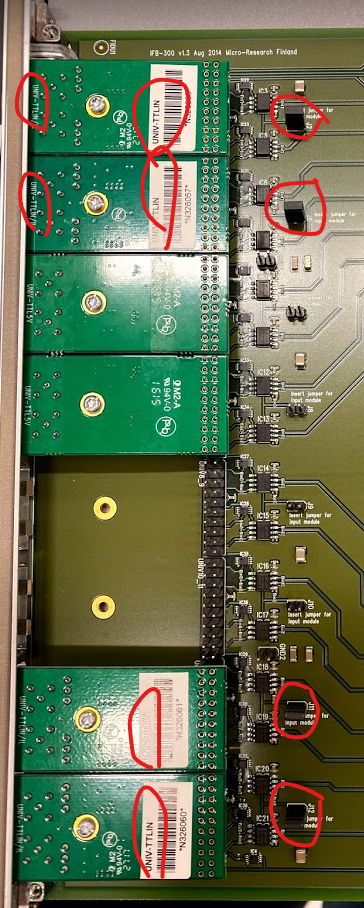
\includegraphics[width=0.5\textwidth]{./pictures/ifb300_test_config.png}
  \caption{IFB-300 populated with input and output modules}
  \label{fig:inputjumpers}
\end{figure}



%\clearpage
\chapter{Troubleshooting}
This chapter hows some errors that can happen when installing and configuring the MRF PCIe-EVR-300DC.\\


\section{PCI error}
If the device file permission is wrong, one can see the following error:
\begin{lstlisting}
mrmEvrSetupPCI("EVR0",  "02:00.0")
Notice: devPCIFindSpec() expect B:D.F in hex
Device EVR0  2:0.0 slot=(null)
Using IRQ 81
Can neither open resource file nor uio file of PCI device 0000:02:00.0 BAR 0
PCI error: Failed to map BARs 0 for EC 30
\end{lstlisting}


\clearpage


%\backmatter

\chapter*{Glossary}\label{sec:glossary}
\addcontentsline{toc}{chapter}{\nameref{sec:glossary}}
\begin{table}[!htb]
%  \footnotesize
%  \centering
  \begin{tabular}{ll}
    \toprule
    \textbf{Term} & Definition                                          \\\midrule
%    AMC           & Advanced Mezzanine Card                             \\
%    CPU           & Central Processing Unit                             \\
%    CU            & Cooling unit                                        \\
    E3            & ESS EPICS environment                               \\
    EPICS         & Experimental Physics and Industrial Control System  \\
    ESS           & European Spallation Source                          \\
    EVM           & Event Master                                        \\
    EVR           & Event Receiver                                      \\
%    FW            & Firmware                                            \\
    FPGA          & Field-Programmable Gate Array                       \\
    ICS           & Integrated Control System                           \\
    I/O           & Input/Output                                        \\
    IOC           & Input/Output Controller                             \\
    IPC           & Industrial PC                                       \\
    MRF           & Micro-Research Finland                               \\
%    PM            & Power module                                        \\
%    RF            & Radio-frequency                                     \\
%    RTM           & Rear Transition Module                              \\
    SFP           & Small Form-factor Pluggable                         \\
    \bottomrule
  \end{tabular}
%  \caption[]{Document revision history.}
  \label{table:glossary}
\end{table}

%\bibliographystyle{unsrt}
%\bibliographystyle{plainnat}
%\bibliographystyle{abbrvnat}
\bibliographystyle{unsrtnat}
%\bibliographystyle{chicago}
\bibliography{ess_refs}

\chapter*{Document revision history}\label{sec:docrevhist}
\addcontentsline{toc}{chapter}{\nameref{sec:docrevhist}}
\begin{table}[!tbh]
  \footnotesize
  \centering
  \begin{tabular}{llll}
    \toprule
    \textbf{Revision} & \textbf{Reason for and description of change} & \textbf{Author}       & \textbf{Date} \\\midrule
    1                 & First release                                 & Javier Cereijo Garcia & \today        \\
    \bottomrule
  \end{tabular}
%  \caption[]{Document revision history.}
  \label{table:docrevhist}
\end{table}


\end{document}
